% Options for packages loaded elsewhere
\PassOptionsToPackage{unicode}{hyperref}
\PassOptionsToPackage{hyphens}{url}
%
\documentclass[
]{article}
\usepackage{lmodern}
\usepackage{amsmath}
\usepackage{ifxetex,ifluatex}
\ifnum 0\ifxetex 1\fi\ifluatex 1\fi=0 % if pdftex
  \usepackage[T1]{fontenc}
  \usepackage[utf8]{inputenc}
  \usepackage{textcomp} % provide euro and other symbols
  \usepackage{amssymb}
\else % if luatex or xetex
  \usepackage{unicode-math}
  \defaultfontfeatures{Scale=MatchLowercase}
  \defaultfontfeatures[\rmfamily]{Ligatures=TeX,Scale=1}
\fi
% Use upquote if available, for straight quotes in verbatim environments
\IfFileExists{upquote.sty}{\usepackage{upquote}}{}
\IfFileExists{microtype.sty}{% use microtype if available
  \usepackage[]{microtype}
  \UseMicrotypeSet[protrusion]{basicmath} % disable protrusion for tt fonts
}{}
\makeatletter
\@ifundefined{KOMAClassName}{% if non-KOMA class
  \IfFileExists{parskip.sty}{%
    \usepackage{parskip}
  }{% else
    \setlength{\parindent}{0pt}
    \setlength{\parskip}{6pt plus 2pt minus 1pt}}
}{% if KOMA class
  \KOMAoptions{parskip=half}}
\makeatother
\usepackage{xcolor}
\IfFileExists{xurl.sty}{\usepackage{xurl}}{} % add URL line breaks if available
\IfFileExists{bookmark.sty}{\usepackage{bookmark}}{\usepackage{hyperref}}
\hypersetup{
  pdftitle={Afleveirng 8},
  hidelinks,
  pdfcreator={LaTeX via pandoc}}
\urlstyle{same} % disable monospaced font for URLs
\usepackage[margin=1in]{geometry}
\usepackage{graphicx}
\makeatletter
\def\maxwidth{\ifdim\Gin@nat@width>\linewidth\linewidth\else\Gin@nat@width\fi}
\def\maxheight{\ifdim\Gin@nat@height>\textheight\textheight\else\Gin@nat@height\fi}
\makeatother
% Scale images if necessary, so that they will not overflow the page
% margins by default, and it is still possible to overwrite the defaults
% using explicit options in \includegraphics[width, height, ...]{}
\setkeys{Gin}{width=\maxwidth,height=\maxheight,keepaspectratio}
% Set default figure placement to htbp
\makeatletter
\def\fps@figure{htbp}
\makeatother
\setlength{\emergencystretch}{3em} % prevent overfull lines
\providecommand{\tightlist}{%
  \setlength{\itemsep}{0pt}\setlength{\parskip}{0pt}}
\setcounter{secnumdepth}{-\maxdimen} % remove section numbering
\ifluatex
  \usepackage{selnolig}  % disable illegal ligatures
\fi

\title{Afleveirng 8}
\usepackage{etoolbox}
\makeatletter
\providecommand{\subtitle}[1]{% add subtitle to \maketitle
  \apptocmd{\@title}{\par {\large #1 \par}}{}{}
}
\makeatother
\subtitle{Lucas Bagge}
\author{}
\date{\vspace{-2.5em}}

\begin{document}
\maketitle

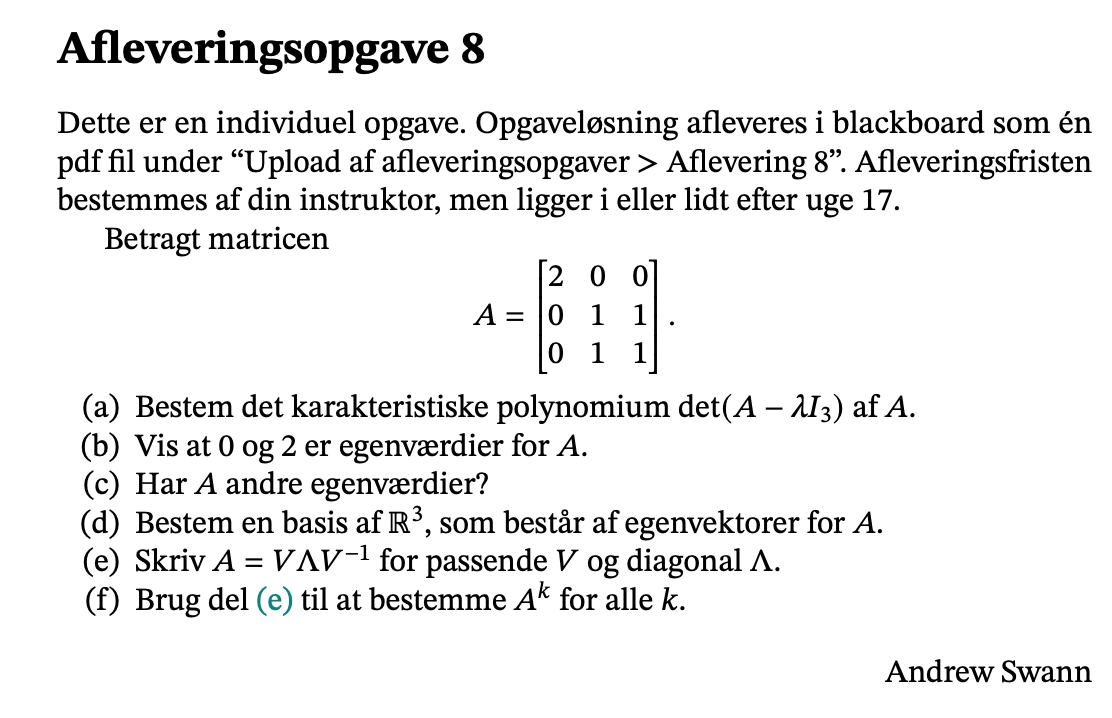
\includegraphics{na.alf.8.png}

\hypertarget{section}{%
\subsubsection{}\label{section}}

\hypertarget{a}{%
\subsubsection{a)}\label{a}}

Vi har følgende matrice:

\[
A=
\begin{pmatrix}
2&0&0\\
0&1&1\\
0&1&1
\end{pmatrix}
\]

Hvor vi vil bestemme det karakteristisk polynomium så vi følger formlen

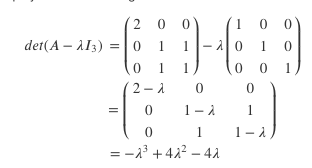
\includegraphics{na.karak.png}

Som er det karakteristisk polynomium for A.

\hypertarget{b}{%
\subsubsection{b)}\label{b}}

Nu skal vi vise at 0 og 2 er egenværdier for A. Det kan vi gøre ved at
løse det karakteristisk polynomium som vi fandt i opgave a:

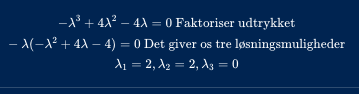
\includegraphics{na.fak.8.png}

\hypertarget{c}{%
\subsubsection{c)}\label{c}}

Ja fra c har jeg vist der er flere en egenværdi mere som er 2.

\hypertarget{d}{%
\subsubsection{d)}\label{d}}

Nu finder vi egenvektorer.

Vi starter med \(\lambda_1=2\)

\[
A=
\begin{pmatrix}
2-2&0&0\\
0&1-2&1\\
0&1&1-2
\end{pmatrix}
\]

\[
A=
\begin{pmatrix}
0&0&0\\
0&-1&1\\
0&1&-1
\end{pmatrix}
\]

Hvor vi skal finde nul rummet. Her skal vi finde echelon form af
ovenstående:

\$\$

\begin{pmatrix}
0&0&0\\
0&-1&1\\
0&1&-1
\end{pmatrix}

\sim

\begin{pmatrix}
0&-1&1\\
0&0&0\\
0&1&-1
\end{pmatrix}

\sim 

\begin{pmatrix}
0&1&-1\\
0&0&0\\
0&1&-1
\end{pmatrix}

\sim

\begin{pmatrix}
0&1&-1\\
0&0&0\\
0&0&0
\end{pmatrix}

\$\$

Herefter skal vi løse følgende:

\[
\begin{pmatrix}
0&1&-1\\
0&0&0\\
0&0&0
\end{pmatrix}
\begin{bmatrix} x_1\\x_2\\x_3 \end{bmatrix}=
\begin{bmatrix} 0\\0\\0 \end{bmatrix}
\]

Dermed får vi

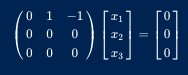
\includegraphics{na.1.8.png}

Dermed er egenvektoren:

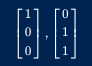
\includegraphics{na.2.8.png}

\end{document}
